\section{Linear Regression Model}

\subsection{One hot encoding}

Linear regression can only operate on numerical values. This caused an issue with the \textbf{Sex} column as it is not numeric. I had to use a technique called "one hot encoding" to transform the Sex column into a usable feature. Interestingly, one hot encoding does not merely transform the sex column into 1 for infant, 2 for male, 3 for female. Instead it creates three new features. These new features are F for female, I for infant and M for male. The feature can have a value of either 1 or 0, 1 meaning "is a" and 0 meaning "not a". For example if F has a value of 1 then we can say it is a female. Alternatively if F has a value of 0 then we can say it is not a female. The results can be seen in figure \ref{fig:abalone-one-hot-encoding}
\begin{figure}[H]
  \centering
  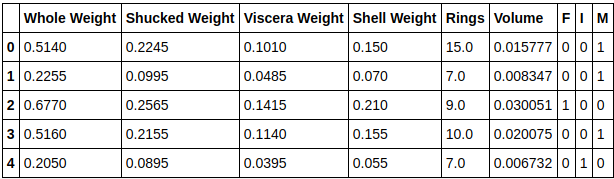
\includegraphics[scale=0.5,width=100mm]{./images/abalone-one-hot-encoding.png}
  \caption{Table showing the results of one hot encoding}
  \label{fig:abalone-one-hot-encoding}
\end{figure}

\subsection{Linear Regression}

\begin{figure}[H]
  \centering
  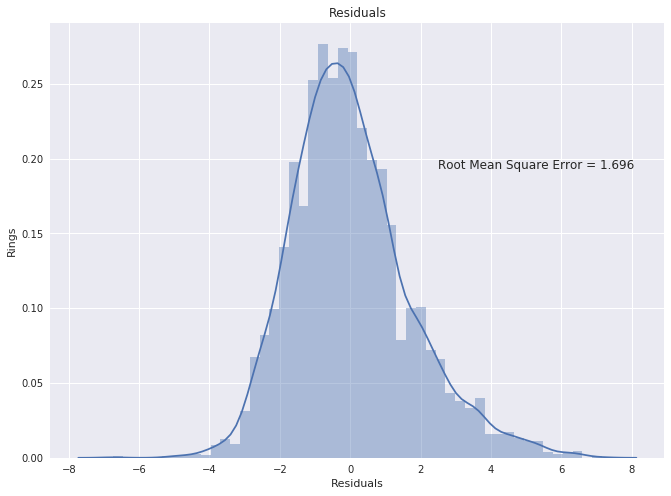
\includegraphics[scale=0.5,width=100mm]{./images/abalone-linear-regression-hist.png}
  \caption{Root mean squared error of  our linear regression}
  \label{fig:abalone-linear-rmse}
\end{figure}

Figure \ref{fig:abalone-linear-rmse} shows a distribution of our residual errors. The residuals seem to follow a fairly normal distribution and our root mean squared error is not bad at 1.69. However our regression score comes out as 0.49. This means that our model will only be correct around 50\% of the time. This is not great.
\begin{figure}[H]
  \centering
  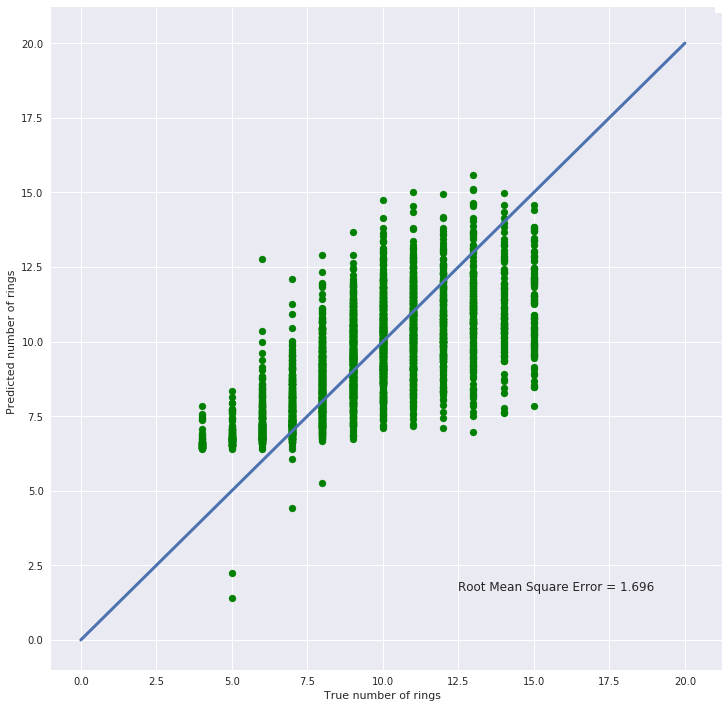
\includegraphics[scale=0.5,width=100mm]{./images/abalone-linear-regression-line.png}
  \caption{Linear regression line for predicting the age of abalones based on the rings}
  \label{fig:abalone-linear-regression-line}
\end{figure}
Figure \ref{fig:abalone-linear-regression-line} shows the linear regression line. From a quick glance the model does not seem to fit our expected value very well. There is a possibility that the sex column may be throwing things off. I shall try plotting a linear regression for each sex. 

\begin{figure}[H]
  \centering
  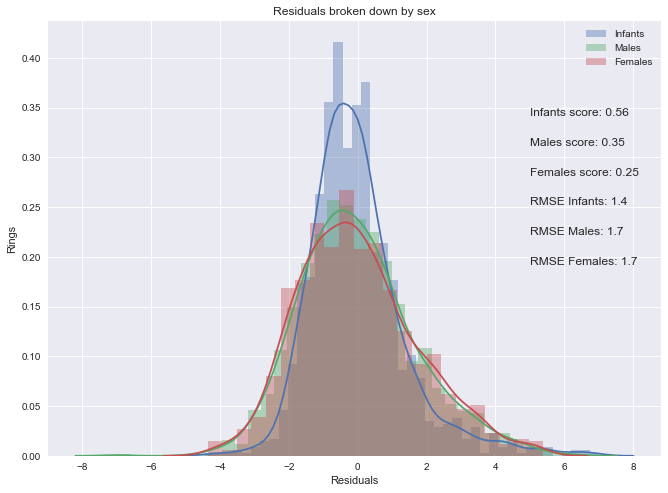
\includegraphics[scale=0.5,width=100mm]{./images/abalone-linear-regression-hist-sex.png}
  \caption{Residuals for values broken down by sex}
  \label{fig:abalone-linear-regression-hist-sex}
\end{figure}

Figure \ref{fig:abalone-linear-regression-hist-sex} seems to indicate that breaking down the values into different sexes does improve the RMSE and the regression score for the infants. However for both male and female our prediction and RMSE seems to have gotten worse. The overall results though are disappointing as 56\% still is not great. Lets check the residuals versus each feature to see if there is any particular feature which may be skewing our results.
\begin{figure}[H]
  \centering
  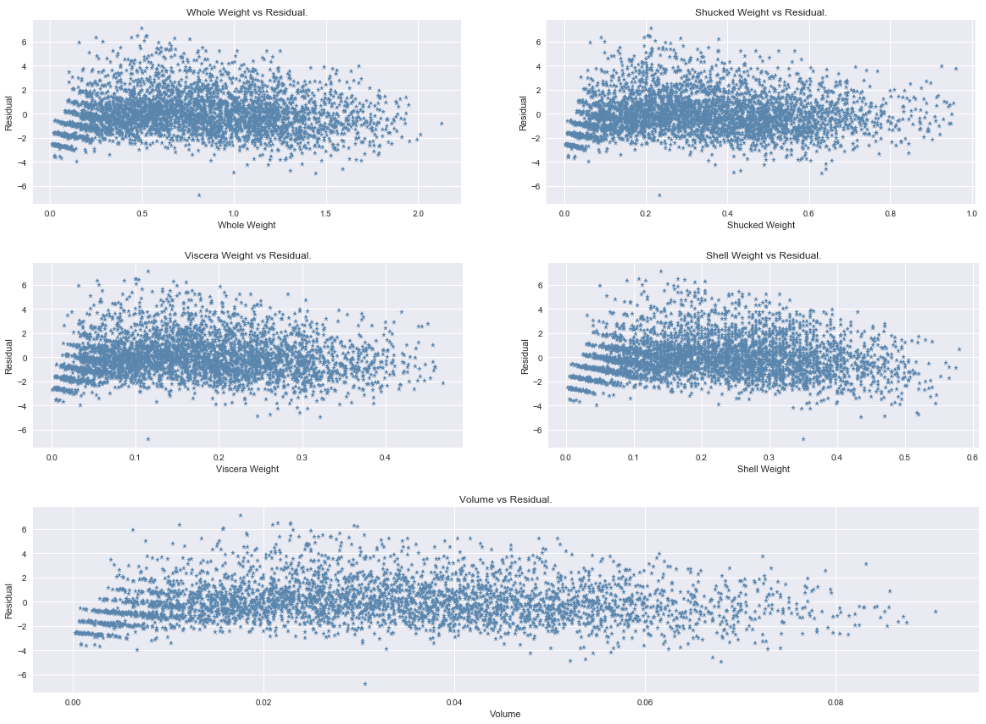
\includegraphics[scale=0.5,width=100mm]{./images/abalone-residuals-vs-features.png}
  \caption{Residuals VS all features}
  \label{fig:abalone-residuals-vs-features}
\end{figure}
The scatter plots seem to indicate that the values are not normally distributed. This means that there may be higher order features that are not accounted for. If this is the case then a linear regression model wont be able to make an accurate prediction. 

\subsection{Lasso}

Lets see if we can improve things using lasso.